%
\againframe{plan}
%
\begin{frame}{Applications of Schr\"odinger's W.E.}
	%
	\[
	\frac{\mathrm{d}^2 \psi(x)}{\mathrm{d} x^2}
	+
	\frac{2m}{\hbar^2}\big(E - V(x)\big) \psi(x)
	=
	0
	\qquad
	\Psi(x, t) = \psi(x) e^{-j \omega t}
	\]
	\hrule
		\begin{itemize}
		\item  The aim is to solve for the time independent wave function $\psi(x)$ for a given potential $V(x)$.
		\item  The potential functions that are useful to describe commonly occurring physical systems are
	\end{itemize}
\end{frame}
%
\begin{frame}{Applications of Schr\"odinger's W.E. (contd...)}
	\begin{footnotesize}
			\begin{table}
			\begin{tabular}{lll}
				\toprule
				\(V(x)\)	&	Name	& 	Physical systems	\\
				\midrule
				0	&	Constant potential	&	Particle in free space	\\
				\midrule
				\(V(x) =  \left\{\begin{array}{ll}
					0	&	0 < x < a	\\
					\infty		&	\text{otherwise}	\\
				\end{array}\right.
				\)	
				&	Infinite potential well	&	Ideal atom	\\
				\midrule
				\(V(x) =  \left\{\begin{array}{ll}
					0	&	-\frac{a}{2} < x < \frac{a}{2}	\\
					V_0		&	\text{otherwise}	\\
				\end{array}\right.
				\)	
				&	Finite potential well	&	Work function	\\
				\midrule
				\(V(x) =  \left\{\begin{array}{ll}
					V_0	&	-\frac{a}{2} < x < \frac{a}{2}	\\
					0		&	\text{otherwise}	\\
				\end{array}\right.
				\)
				&	Finite barrier	&	Nuclear fission	\\
				&	&	Scanning Tunneling 	\\
				&	&	Microscope	\\
				\bottomrule
			\end{tabular}
		\end{table}
	\end{footnotesize}
\end{frame}
%
\begin{frame}
	\begin{huge}
		\begin{center}
			Particle in free space
		\end{center}
	\end{huge}
\end{frame}
%
\begin{frame}{\(V(x) :\) Constant potential }
	%
	\[
	\frac{\mathrm{d}^2 \psi(x)}{\mathrm{d} x^2}
	+
	\frac{2mE}{\hbar^2} \psi(x)
	=
	0
	\qquad
	\Psi(x, t) = \psi(x) e^{-j \omega t}
	\]
	\hrule
	%
	\begin{itemize}
		\item Let us define the wave vector \(k\) as
		\[
		k = \sqrt{\frac{2mE}{\hbar^2}}
		\]
		so that the Time Independent Schr\"odinger Equation (TISE) is reduced to 
		\[
		\frac{\mathrm{d}^2 \psi(x)}{\mathrm{d} x^2}
		+
		k^2 \psi(x)
		=
		0
		\]
		so that
		\[
		\frac{\mathrm{d}^2 \psi(x)}{\mathrm{d} x^2}  = - k^2 \psi(x)
		\]
	\end{itemize}
\end{frame}
%
\begin{frame}{\(V(x) :\) Constant potential -- Solution of TISE}
	%
	\[
	\frac{\mathrm{d}^2 \psi(x)}{\mathrm{d} x^2}  = - k^2 \psi(x)
	\]
	\hrule
	%
	%
	\begin{itemize}
		\item The solution of above differential equation can be written as
		\[
		\psi(x)  = A e^{j k x} + B e^{-j k x}
		\]
		\item If we use the Euler's formula
		\[
		e^{j x} = \cos x + j \sin x 
		\]
		then the solution can be written also as
		\[
		\psi(x)  = A' \cos k x + B' \sin k x
		\]
	\end{itemize}
\end{frame}
%
\begin{frame}{\(V(x) :\) Constant potential -- Wave vector, Momentum and Energy}
	\begin{itemize}
		\item All the wave vectors are allowed
		\[
		k = -\infty \, \text{to} +\infty
		\]
		\item The momentum is given by
		\[
		p = \frac{h}{\lambda} \Rightarrow p = \hbar k \qquad \qquad[\because k = \frac{2\pi}{\lambda}]
		\]
		\item The corresponding energy levels are given by
		\[
		E = \frac{p^2}{2m} = \frac{\hbar^2 k^2}{2m}
		\]
	\end{itemize}
\end{frame}
%
\begin{frame}{\(V(x) :\) Constant potential -- Solution of TDSE}
	\begin{itemize}
		\item The solution of Time Dependent part of Schr\"odinger Equation (TDSE) is given by
		\[
		\phi(t) = e^{-j \omega t}, \qquad \text{where} \qquad \omega = \frac{E}{\hbar} = \frac{\hbar k^2}{2 m}
		\]
		\item The total wave function is given by
		\[
		\Psi_k(x, t) = \psi_k(x)\phi_k(t) = e^{j\overline{k x - \omega t}}.
		\]
		where the subscript \(k\) is the quantum number.
	\end{itemize}
\end{frame}
\begin{frame}{\(V(x) :\) Constant potential -- Nature of solutions}
	%
	\begin{itemize}
		\item The solutions are \textbf{traveling} waves.
		\item The energy \(E\) can be any positive real number and is related to the wave vector \(k\) by
		\[
		E = \frac{\hbar^2 k^2}{2m}
		\]
	\end{itemize}
	%
	\begin{figure}
		
\includegraphics[width=0.8\textwidth]{qm_constant_potential_travelling_waves_solution}
	\end{figure}
\end{frame}
%
\begin{frame}{Constant potential: problems}
	\begin{problem}
		An electron in free space is described by a plane wave given by 
		\(\Psi(x,t) = A \exp(j(kx -\omega t))\). If \(k = \SI{8e8}{\per\metre}\) and \(\omega = \SI{8e12}{\radian\per\second}\), determine
		\begin{enumerate}
			\item phase velocity and wavelength of the plane wave
			\item momentum and kinetic energy (in \si{\electron\volt})
		\end{enumerate}
		%
		Repeat the steps for \(k = -\SI{1.5e9}{\per\metre}\) and \(\omega = \SI{1.5e13}{\radian\per\second}\).
	\end{problem}
	%
	\begin{problem}
		Determine the wave number, wavelength, angular frequency, and period of wavefunction that describes an electron traveling in free space at a velocity of (a) \SI{5e6}{\centi\metre\per\second}.
	\end{problem}
\end{frame}
%
\begin{frame}{Summary of particle in free space}
	\begin{itemize}
		\item For a particle in free space, all wave vectors are allowed 
		\(
		k = -\infty \, \text{to} +\infty
		\).
		\item The corresponding energy levels are given by
		\[
		E = \frac{p^2}{2m} = \frac{\hbar^2 k^2}{2m}
		\]
		\item The time independent part of wave function is given by
		\[
		\psi(x) = e^{j k x}
		\]
		\item The time dependent part of wave function is given by
		\[
		\phi(t) = e^{-j \omega t}, \qquad \text{where} \qquad \omega = \frac{E}{\hbar}
		\]
		\item The total wave function is given by
		\[
		\Psi_k(x, t) = \psi_k(x)\phi_k(t) = e^{j\overline{k x - \omega t}}.
		\]
	\end{itemize}
\end{frame}
%
\begin{frame}
	\begin{huge}
		\begin{center}
			*Particle in a 1D box*
		\end{center}
	\end{huge}
\end{frame}
%
\begin{frame}{\(V(x) :\) Infinite potential}
	%
	\begin{columns}
		%
		\begin{column}{0.6\textwidth}
			\[
			V(x) =  \left\{\begin{array}{ll}
				0	&	0 < x < a	\\
				\infty		&	\text{otherwise}	\\
			\end{array}\right.
			\]
		\end{column}
		%
		\begin{column}{0.38\textwidth}
			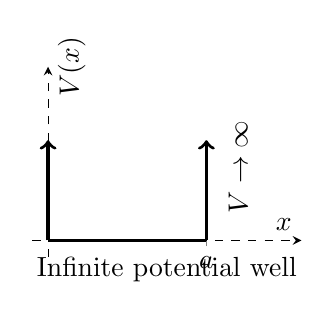
\begin{tikzpicture}
				\def\w{5.0cm}   % width of each plot
				\def\h{4.0cm}   % height of each plot
				
				% ---------- 1) Infinite potential well ----------
				\begin{axis}[
					at={(0,0)},
					anchor=south west,
					width=\w,height=\h,
					axis lines=middle,
					xmin=-0.2, xmax=3.2,
					ymin=-0.5, ymax=5.2,
					xtick={0,2},
					xticklabels={\(0\), \( a\)},
					x axis line style={dashed}, % make x-axis dashed
					y axis line style={dashed}, % make y-axis dashed
					ytick={0},
					xlabel={$x$},
					ylabel={$V(x)$},
					ylabel style={rotate=90},
					title={Infinite potential well},
					every axis title/.style={at={(0.5,0.05)},anchor=north},
					clip=false
					]
					% well bottom (zero inside)
					\addplot[very thick,domain=0:2,samples=2] ({x},{0});
					% outside near-infinite walls: plot big vertical lines
					%\addplot[very thick] coordinates {(-1,0) (-1,5)};
					\draw[->, very thick](0,0) -- (0,3);
					\draw[->, very thick](2,0) -- (2,3);
					% annotate "infinite" label
					\node[anchor=west, rotate=90] at (axis cs:2.4,0.5) {\(\displaystyle V\to\infty\)};
				\end{axis}
			\end{tikzpicture}
		\end{column}
	\end{columns}
	\hrule
	%
	\begin{itemize}
		\item Consider a particle in a 1-dimensional infinite potential well.
		\item The well can be considered as a box.
	\end{itemize}
	%
	\begin{columns}[t]
		\begin{column}[t]{0.5\textwidth}
			\begin{center}
				Outside infinite box
			\end{center}
			%
			\[
			\frac{\mathrm{d}^2 \psi(x)}{\mathrm{d} x^2}
			+
			\frac{2m}{\hbar^2}\big(E -\infty\big) \psi(x)
			=
			0	
			\]
			%
		\end{column}
		%
		\begin{column}[t]{0.48\textwidth}
			\begin{center}
				Inside infinite box
			\end{center}
			%
			\[
			\frac{\mathrm{d}^2 \psi(x)}{\mathrm{d} x^2}
			+
			\frac{2mE}{\hbar^2} \psi(x)
			=
			0
			\]
			%
		\end{column}
	\end{columns}
	%
\end{frame}
%
\begin{frame}{\(V(x) :\) Infinite potential well -- Solution of TISE}
	%
	\begin{columns}[t]
		\begin{column}[t]{0.5\textwidth}
			\begin{center}
				Outside infinite box
			\end{center}
			%
			\begin{itemize}
				\item There is no wave function!
				\[
				\psi(x) = 0 
				\]
			\end{itemize}
		\end{column}
		%
		\begin{column}[t]{0.48\textwidth}
			\begin{center}
				Inside infinite box
			\end{center}
			%
			\begin{itemize}
				\item The wavefunction is
				\[
				\psi(x)  = A \cos k x + B \sin k x
				\]
			\end{itemize}
		\end{column}
	\end{columns}
	%
	\begin{itemize}
		\item Upon applying boundary conditions
	\end{itemize}
	%
	\begin{columns}[t]
		\begin{column}[t]{0.5\textwidth}
			\begin{center}
				Left B.C.
			\end{center}
			%
			\begin{align*}
				\psi(x=0) &= 0	\\
				A \cos k x &= 0 \\
				\Rightarrow A &= 0
			\end{align*}
		\end{column}
		%
		\begin{column}[t]{0.48\textwidth}
			\begin{center}
				Right B.C.
			\end{center}
			%
			\begin{align*}
				\psi(x=a) &= 0 \\
				B \sin k a &= 0 \\
				\Rightarrow \sin k a &= 0
			\end{align*}
		\end{column}
	\end{columns}
	%
\end{frame}
%
\begin{frame}{\(V(x) :\) Infinite potential well -- Solution of TISE}
	%
\begin{footnotesize}
		\begin{itemize}
		\item The equation \(\sin k a = 0\) is valid if
		\[
		ka = n\pi
		\]
		where n is a positive integer, or \(n = 1, 2, 3, \ldots\). The parameter is referred to as quantum number. In terms of the quantum number, the wave vector is given by
		\[
		k = \frac{n\pi}{a}
		\]
		\item The prefactor \(B\) can be found by applying the \textbf{normality condition} of wave function.
		\[
		\int_{0}^{a} |B \sin k x|^2 \, \mathrm{d}x = 1, \qquad \Rightarrow \qquad \int_{0}^{a} B^2 \sin^2 k x \, \mathrm{d}x = 1
		\]
		\[
		\therefore B = \sqrt{\frac{2}{a}}
		\]
		\item Therefore, the time independent wave function is given by
		\[
		\psi_n(x) = \sqrt{\frac{2}{a}} \sin\left(\frac{n\pi x}{a}\right)
		\]
	\end{itemize}
\end{footnotesize}
	%
\end{frame}
%
\begin{frame}{\(V(x) :\) Infinite potential well -- Energy levels}
	\begin{itemize}
		\item Recall that the wave vector \(k\) is related to the energy \(E\) by
		\[
		k = \sqrt{\frac{2mE}{\hbar^2}}, \qquad \Rightarrow \qquad E = \frac{\hbar^2 k^2}{2m}
		\]
		\item Therefore, the energy is given by
		\[
		E = E_n = \frac{n^2\hbar^2\pi^2}{2ma^2}
		\]
	\end{itemize}
	%
	\begin{problem}
		Electron in an infinite potential well of width \SI{5}{\angstrom}. Calculate the first three energy levels.
	\end{problem}
	\begin{keyinsight}
		The energy of particle is \textbf{quantized} i.e. it can only have particular \textbf{discrete} values.
	\end{keyinsight}
\end{frame}
%
\begin{frame}{\(V(x) :\) Infinite potential well -- Nature of solutions}
	%
	\begin{itemize}
		\item The solutions are \textbf{standing} waves.
	\end{itemize}
	\begin{figure}
		
\includegraphics[width=0.8\textwidth]{qm_infinite_potential_well_solution}
	\end{figure}
\end{frame}
%
\begin{frame}{Orthogonality condition}
	\begin{itemize}
		\item Wave function associated with an energy level is normalized.
		\item In addition to normality,  wave functions \(\psi_m(x), \psi_n(x)\) corresponding to any two levels \(m, n\) of infinite potential well are orthogonal to each other i.e.
		\[
		\int_{0}^{a} \psi_m^*(x) \psi_n(x) \, \mathrm{d}x = 0.
		\]
		This is called the \textbf{orthogonality condition}.
	\end{itemize}
	%
	\begin{theorem}
		Prove the orthogonality condition for solutions of infinite potential well.
	\end{theorem}
\end{frame}
%
\begin{frame}{1D infinite well: problems}
	\begin{problem}
		\begin{enumerate}
			\item A particle with mass of \SI{15}{\milli\gram} is bound in a 1D infinte potential well that is \SI{1.2}{\centi\metre} wide.
			\item If the energy of the particle is \SI{15}{\milli\joule}, determine the value of n for that state.
			\item What is the energy of the \((n+1)\) state?
			\item Would quantum effects be observable for this particle?
		\end{enumerate}
	\end{problem}
	%
\end{frame}
%
\begin{frame}{Summary of particle in infinite potential well}
	%
	\begin{itemize}
		\item For a particle in an infinite potential well, discrete wave vectors are allowed and are given by
		\[
		k_n = \frac{n\pi}{a}.
		\]
		\item The corresponding energy levels are given by
		\[
		E_n = \frac{\hbar^2 k^2}{2m}, \qquad \text{or} \qquad E_n = \frac{n^2\hbar^2\pi^2}{2ma^2}
		\]
		\item The time independent part of wave function is given by
		\[
		\psi_n(x) = \sqrt{\frac{2}{a}} \sin\left(\frac{n\pi x}{a}\right)
		\]
		\item The time dependent part of wave function is given by
		\[
		\phi_n(t) = e^{-j\omega_n t}, \qquad \text{where} \qquad \omega_n = \frac{E_n}{\hbar}
		\]
		\item The total wave function is given by
		\[
		\Psi_n(x, t) = \psi_n(x)\phi_n(t),
		\]
	\end{itemize}
\end{frame}
%
\begin{frame}
	\begin{huge}
		\begin{center}
			*Particle in a symmetric form infinite potential well*
		\end{center}
	\end{huge}
\end{frame}
%
%
\begin{frame}{\(V(x) :\) Symmetric Infinite potential}
	%
	\begin{columns}
		%
		\begin{column}{0.6\textwidth}
			\[
			V(x) =  \left\{\begin{array}{ll}
				0	&	-\frac{a}{2} \leq x \leq +\frac{a}{2}	\\
				\infty		&	\text{otherwise}	\\
			\end{array}\right.
			\]
		\end{column}
		%
		\begin{column}{0.38\textwidth}
			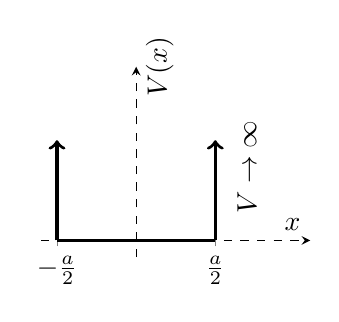
\begin{tikzpicture}
				\def\w{5.0cm}   % width of each plot
				\def\h{4.0cm}   % height of each plot
				
				% ---------- 1) Symmetric Infinite potential well ----------
				\begin{axis}[
					at={(0,0)},
					anchor=south west,
					width=\w,height=\h,
					axis lines=middle,
					xmin=-1.2, xmax=2.2,
					ymin=-0.5, ymax=5.2,
					xtick={-1,1},
					xticklabels={\(-\frac{a}{2}\), \( \frac{a}{2}\)},
					x axis line style={dashed}, % make x-axis dashed
					y axis line style={dashed}, % make y-axis dashed
					ytick={0},
					xlabel={$x$},
					ylabel={$V(x)$},
					ylabel style={rotate=90},
					%title={Symmetric},
					every axis title/.style={at={(0.5,0.05)},anchor=north},
					clip=false
					]
					% well bottom (zero inside)
					\addplot[very thick,domain=-1:1,samples=2] ({x},{0});
					% outside near-infinite walls: plot big vertical lines
					%\addplot[very thick] coordinates {(-1,0) (-1,5)};
					\draw[->, very thick](-1,0) -- (-1,3);
					\draw[->, very thick](1,0) -- (1,3);
					% annotate "infinite" label
					\node[anchor=west, rotate=90] at (axis cs:1.4,0.5) {\(\displaystyle V\to\infty\)};
				\end{axis}
			\end{tikzpicture}
		\end{column}
	\end{columns}
	\hrule
	%
	\begin{itemize}
		\item Consider a particle in a \textbf{symmetric form} of 1-dimensional infinite potential well.
		\item The analysis for this potential is similar to the analysis for the asymmetric form discussed earlier.
		\item However, the general form of wave function can be considered as linear combination of exponential functions instead of trigonometric functions due to the symmetry of the problem.
		\item Thus, let the wave function inside the well be
		\[
		\psi(x)  = A e^{j k x} + B e^{-j k x}
		\]
	\end{itemize}
	%
\end{frame}
%
\begin{frame}{\(V(x) :\) Symmetric Infinite potential -- Solution of TISE}
	%
	\[
	\psi(x)  = A e^{j k x} + B e^{-j k x}
	\]
	\hrule
	%
	\begin{itemize}
		\item Upon applying left boundary condition,
		\begin{align*}
			&\phantom{\Leftrightarrow}\psi(x=-\frac{a}{2}) = 0	\\
			&\Leftrightarrow A \exp\big(-j  \frac{ka}{2}\big) + B \exp\big(+j  \frac{ka}{2}\big) =0 \\
			&\Leftrightarrow (A+B)\cos \big( \frac{ka}{2}\big) + j (-A+B) \sin \big( \frac{ka}{2}\big) = 0\\
			& \Leftrightarrow (A+B)\cos \big( \frac{ka}{2}\big) = 0 \, \text{and} \, (-A+B) \sin \big( \frac{ka}{2}\big) = 0 \\
			& \Leftrightarrow \big[A+B = 0 \, \text{or} \, \cos \big( \frac{ka}{2}\big) = 0\big] \, \text{and} \, \big[A-B=0 \, \text{or} \, \sin \big( \frac{ka}{2}\big) = 0\big]	\\
			& \Leftrightarrow \big[A-B=0  \, \text{and} \, \cos \big( \frac{ka}{2}\big) = 0\big] \, \text{or} \,  \big[A+B = 0 \, \text{and} \, \sin \big( \frac{ka}{2}\big) = 0\big]
		\end{align*}
		%
		\item Same cases arise for the right boundary condition due to \textbf{symmetry} of the problem!
	\end{itemize}
\end{frame}
%
\begin{frame}{\(V(x) :\) Symmetric Infinite potential -- Solution of TISE}
	%
	\[
	\psi(x)  = A e^{j k x} + B e^{-j k x}
	\]
	\hrule
	%
	\begin{center}
		Case (i) Even wave functions
	\end{center}
	%
	\vspace{-5ex}
	%
	\begin{columns}[t]
		\begin{column}[t]{0.4\textwidth}
			%
			\begin{align*}
				\phantom{\Leftrightarrow} A-B &= 0	\\
				\Leftrightarrow \psi(x)  &= A \cos k x
			\end{align*}
			%
		\end{column}
		%
		\begin{column}{0.18\textwidth}
			\begin{center}
				and
			\end{center}
		\end{column}
		%
		\begin{column}[t]{0.4\textwidth}
			%
			\begin{align*}
				\cos \big( \frac{ka}{2}\big) &= 0	\\
				\Leftrightarrow	\frac{ka}{2} &= \frac{\pi}{2}, \frac{3\pi}{2}, \ldots	\\
				\Leftrightarrow	k &= \frac{\pi}{a}, \frac{3\pi}{a}, \ldots
			\end{align*}
		\end{column}
	\end{columns}
	%
	\begin{center}
		Case (ii) Odd wave functions
	\end{center}
	%
	\vspace{-5ex}
	%
	\begin{columns}[t]
		\begin{column}[t]{0.4\textwidth}
			%
			\begin{align*}
				\phantom{\Leftrightarrow} A+B &= 0	\\
				 \Leftrightarrow \psi(x)  &= A \sin k x
			\end{align*}
			%
		\end{column}
		%
		\begin{column}{0.18\textwidth}
			\begin{center}
				and
			\end{center}
		\end{column}
		%
		\begin{column}[t]{0.4\textwidth}
			%
			\begin{align*}
				\sin \big( \frac{ka}{2}\big) &= 0	\\
				\Leftrightarrow	 \frac{ka}{2} &= \pi, 2\pi, \ldots \\
				\Leftrightarrow	k &= \frac{2\pi}{a}, \frac{4\pi}{a}, \ldots
			\end{align*}
		\end{column}
	\end{columns}
\end{frame}
%
\begin{frame}{\(V(x) :\) Symmetric Infinite potential -- Nature of solutions}
%
\begin{columns}
	\begin{column}{0.7\textwidth}
			%
	\[
	f(x) := 
	\left\{
	\begin{array}{ll}
		\text{even} &	\text{if} \quad f(-x) = f(x)	\\
		\text{odd} &	\text{if} \quad f(-x) = -f(x)	\\
	\end{array}
	\right.
	\]
	\end{column}
	%
	\begin{column}{0.28\textwidth}
		%
		
\includegraphics[width=\textwidth]{qm_schrodinger_equation_even_odd_function}
	\end{column}
	%
\end{columns}
%
\hrule
%
\begin{columns}
	\begin{column}{0.70\textwidth}
			%
\begin{footnotesize}
		\begin{itemize}
		\item The potential function is an even function as \(V(-x)= V(x)\).
		\item The wave functions belonging to first case are even functions as \(\cos x\) is an even function whereas the wave functions belonging to second case are odd functions as \(\sin x\) is an odd function.
		\item There are two subfamilies of even and odd wave functions
		\item If we order the wave functions with increasing wave vector, then wave functions alternate between even and odd.
	\end{itemize}
\end{footnotesize}
	\end{column}
	%
	\begin{column}{0.28\textwidth}
		%
		
\includegraphics[width=0.9\textwidth]{qm_schrodinger_equation_symmetric_potential_well_solutions}
	\end{column}
\end{columns}
\end{frame}
%
\begin{frame}{\(V(x) :\) Symmetric Infinite potential -- Alternative solution}
	%
	\begin{columns}
		\begin{column}{0.7\textwidth}
			%
			\begin{itemize}
				\item Translation of origin by \(\alpha\) transforms the function in new coordinate frame
			\end{itemize}
			\[
			f^{\text{new}}(x) = f^{\text{old}}(x + \alpha)
			\]
		\end{column}
		%
		\begin{column}{0.28\textwidth}
			%
			
\includegraphics[width=\textwidth]{qm_schrodinger_equation_translation_axes}
		\end{column}
		%
	\end{columns}
	\hrule
	%
	\begin{itemize}
		\item The solutions to the symmetric form of infinite potential well can be obtained from the solutions to the asymmetric form by translating the coordinate frame by \(\tfrac{a}{2}\).
		\[
		x \rightarrow x + \frac{a}{2}
		\]
		\item The wave functions of the symmetric potential well are given by
		\[
		\psi^\text{sym}(x) = \psi^\text{asym}(x + \frac{a}{2})
		\]
		\begin{align*}
			\psi^\text{sym}(x) &= \psi^\text{asym}(x + \frac{a}{2})	\\
			&= \sqrt{\frac{2}{a}} \sin\left(\frac{n\pi}{a} \overline{x + \frac{a}{2}}\right)	= \sqrt{\frac{2}{a}}  \sin\left(\frac{n\pi x}{a} + \frac{n\pi}{2} \right)
		\end{align*}
	\end{itemize}
\end{frame}
%
\begin{frame}{\(V(x) :\) Symmetric Infinite potential -- Alternative solution}
%
\begin{columns}
	\begin{column}{0.4\textwidth}
		\begin{itemize}
			\item Upon substituting for \(n=1,2,\ldots\), we have
			\item Using the trigonometric relations, we have
			\item In some cases, prefactor of \(-1\) can be absorbed into normalizing factor.
			\item Thus, the solutions are grouped into even and odd families.
		\end{itemize}
		%
	\end{column}
	%
	\begin{column}{0.58\textwidth}
		\begin{itemize}
			\item 
			\[
			\psi^\text{sym}(x) \propto
			\left\{
			\begin{array}{ll}
				\sin\left(\frac{\pi x}{a} + \frac{\pi}{2} \right)	&	n=1	\\
				\sin\left(\frac{2\pi x}{a} + \frac{2\pi}{2} \right)	&	n=2	\\
				\sin\left(\frac{3\pi x}{a} + \frac{3\pi}{2} \right)	&	n=3	\\
				\sin\left(\frac{4\pi x}{a} + \frac{4\pi}{2} \right)	&	n=4	\\
				\vdots	&	\vdots
			\end{array}
			\right.
			\]
			\item 
			\[
			\psi^\text{sym}(x) \propto
			\left\{
			\begin{array}{ll}
				\cos\left(\frac{\pi x}{a}\right)	&	n=1	\\
				\sin\left(\frac{2\pi x}{a} \right)	&	n=2	\\
				\cos\left(\frac{3\pi x}{a} \right)	&	n=3	\\
				\sin\left(\frac{4\pi x}{a} \right)	&	n=4	\\
				\vdots	&	\vdots
			\end{array}
			\right.
			\]
		\end{itemize}
		%
	\end{column}
\end{columns}
%
\end{frame}
%
\begin{frame}{Summary of particle in symmetric infinite potential well}
	\begin{itemize}
		\item For a particle in a symmetric infinite potential well, the allowed wave vectors are same as that of asymmetric infinite potential well.
		\item The corresponding energy levels are also same
		\item The potential well function is an even function i.e.
		\[
		V(-x) = V(x).
		\]
		Due to the symmetry of the potential well function, the wave functions are either \textbf{odd} or \textbf{even}.
	\end{itemize}
\end{frame}
%
%
\begin{frame}
	\begin{huge}
		\begin{center}
			*Particle in a finite potential well*
		\end{center}
	\end{huge}
\end{frame}
%
\begin{frame}{Potential energy barrier -- Classical vs Quantum}
	%
	\begin{figure}
		
\includegraphics[width=0.3\textwidth]{qm_schrodinger_equation_energy_barrier_classical_particle}
		
\includegraphics[width=0.3\textwidth]{qm_schrodinger_equation_energy_barrier_quantum_particle}
	\end{figure}
	%
	\begin{itemize}
		\item There are two regions -- (I) without barrier and (II) with barrier
	\end{itemize}
	%
	\vspace{-1em}
	%
	\begin{block}{Region I}
		\begin{itemize}
			\item Total energy \(E\) is kinetic energy \(T_\text{I}\) \hfill
			%
			\(
			T_\text{I} = E
			\)
			\item Wave vector is real \hfill
			\(
			k_\text{I} = \sqrt{\frac{2mT_\text{I}}{\hbar^2} }
			\)
			\item Wave function has sinusoidal form \hfill
			\(
			\psi_\text{I}(x) = A \exp j k_\text{I} x + B \exp - j k_\text{I} x
			\)
		\end{itemize}
	\end{block}
	%
	\vspace{-1em}
	%
\begin{block}{Region II}
	\begin{itemize}
	\item There are two cases -- (i) total energy is greater than potential energy barrier and (ii)  total energy is lesser than potential energy barrier.
\end{itemize}
\end{block}
\end{frame}
%
\begin{frame}{Case (i) -- \(E > V_0\)}
	%
	\begin{itemize}
	\item Classically, the particle overcomes the potential barrier with decreased kinetic energy. 
	\item Quantum mechanically, the particle overcomes the potential barrier with decreased wave vector.
\end{itemize}
	%
\begin{footnotesize}
		\begin{block}{Region II}
		\begin{itemize}
			%
			\item Kinetic energy is reduced by \(V_0\) \hfill
			\(
			T_\text{II} = E - V_0
			\)
			\item The wave function is given by
			\[
			\frac{\mathrm{d}^2 \psi(x)}{\mathrm{d} x^2}
			+
			\frac{2m(E- V_0)}{\hbar^2} \psi(x)
			=
			0
			\]
			\item Wave vector is real
			\[
			k_\text{II} = \sqrt{\frac{2m(E - V_0)}{\hbar^2} }
			\]
			\item Wave vector is reduced compared to region I
			\item Wave function has sinusoidal form \hfill
			\(
			\psi_\text{II}(x) = A \exp j k_\text{II} x + B \exp - j k_\text{II} x
			\)
		\end{itemize}
	\end{block}
\end{footnotesize}
\end{frame}
%
\begin{frame}{Curious case -- \(E < V_0\)}
	%
	\begin{itemize}
		\item \colorbox{red}{Classically, the particle \textbf{cannot} overcome the potential barrier.}
		\item \colorbox{green}{However, quantum mechanically, it is possible!}
		\item \colorbox{yellow}{Negative kinetic energy is allowed in quantum mechanics.}
	\end{itemize}
\begin{footnotesize}
		\begin{block}{Region II}
		\begin{itemize}
			\item Total energy \(E\) is less than potential barrier
			%
			\item Kinetic energy is negative! \hfill
			\(
			T_\text{II} = E - V_0 < 0
			\)
			\item Wavevector is imaginary
			\[
			k_\text{II} = \sqrt{\frac{2m(E - V_0)}{\hbar^2}} = j  \sqrt{\frac{2m(V_0 - E)}{\hbar^2}} = j \kappa_\text{II}
			\]
			\item Wave function has exponential form
			%
			\begin{align*}
				\psi_\text{II}(x) &= A \exp j k_\text{II} x + B \exp - j k_\text{II} x	\\
				&= A \exp - \kappa_\text{II} x + B \exp + \kappa_\text{II} x
			\end{align*}
		\end{itemize}
	\end{block}
\end{footnotesize}
\end{frame}
%
\begin{frame}{\(V(x) :\) Finite potential well}
	%
	\begin{columns}
		%
		\begin{column}{0.6\textwidth}
			\[
			V(x) =  \left\{\begin{array}{ll}
				0	&	-\frac{a}{2} < x < \frac{a}{2}	\\
				V_0		&	\text{otherwise}	\\
			\end{array}\right.	
			\]
		\end{column}
		%
		\begin{column}{0.38\textwidth}
			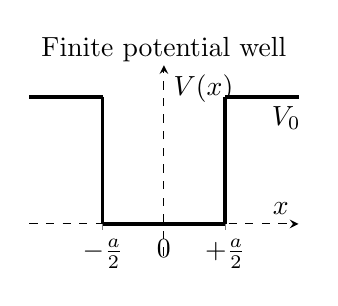
\begin{tikzpicture}
				\def\w{5.0cm}   % width of each plot
				\def\h{4.0cm}   % height of each plot
				
				% ---------- 2) Finite potential well ----------
				\begin{axis}[
					at={(6.2cm,0)}, anchor=south west,
					width=\w,height=\h,
					axis lines=middle,
					xmin=-2.2, xmax=2.2,
					ymin=-0.5, ymax=2.5,
					xtick={-1,1},
					xticklabels={\( -\frac{a}{2}\), \( +\frac{a}{2}\)},
					x axis line style={dashed}, % make x-axis dashed
					y axis line style={dashed}, % make y-axis dashed
					ytick=\empty,     % removes both ticks and labels
					%yticklabels={0,$-V_0$},
					xlabel={$x$},
					ylabel={$V(x)$},
					title={Finite potential well},
					every axis title/.style={at={(0.5,1.2)},anchor=north},
					clip=false
					]
					% outside region: V = V_0
					\addplot[very thick,domain=-2.2:-1,samples=2] ({x},{2});
					\addplot[very thick,domain=1:2.2,samples=2] ({x},{2});
					% inside: negative finite well depth (e.g. -2)
					\addplot[very thick] coordinates {(-1,0) (1,0)};
					% vertical steps at boundaries
					\addplot[very thick] coordinates {(-1,2) (-1,0)};
					\addplot[very thick] coordinates {(1,2) (1,0)};
					% label
					\node[anchor=north] at (axis cs:2,2) {\(\displaystyle V_0\)};
					\node[anchor=north] at (axis cs:0,-0.1) {\(\displaystyle 0\)};
				\end{axis}
			\end{tikzpicture}
		\end{column}
	\end{columns}
	\hrule
	%
	\begin{itemize}
		\item There are three regions -- (I) well, (II) right of well, and (III) left of well.
		\item There are two cases -- (i) total energy is less than potential barrier and (ii)  total energy is greater than potential barrier
		\item Let us solve for case (i).
	\end{itemize}
\end{frame}
%
\begin{frame}{\(V(x) :\) Finite potential well -- Case (i): \(E < V_0\)}
\begin{footnotesize}
		\begin{block}{Region I}
		\begin{itemize}
			\item Kinetic energy is positive so \hfill
			\(
			\psi_\text{I}(x) = A \exp (j k_\text{I} x) + B \exp (- j k_\text{I} x)
			\)
			\item Apply the \textbf{symmetry condition} of even or odd wave function
			\[
			\text{Case (1):} \, A = B \quad \text{or} \quad \text{Case (2):} \, A=-B
			\]
		\end{itemize}
	\end{block}
\end{footnotesize}
	%
	\vspace{-4ex}
	%
\begin{footnotesize}
	\begin{columns}
	\begin{column}[t]{0.5\textwidth}
		\begin{block}{Region II}
			\begin{itemize}
				\item Kinetic energy is negative so
				\[
				\psi_\text{II}(x) = C \exp (- \kappa_\text{II} x) + D \exp (+ \kappa_\text{II} x)
				\]
				\item Apply the \textbf{finiteness condition}
				\begin{align*}
					&\phantom{\Leftrightarrow}\lim_{x\rightarrow \infty} \psi_\text{II}(x) = \, \text{finite} \\
					&\Leftrightarrow D=0.
				\end{align*}
			\end{itemize}
		\end{block}
	\end{column}
	%
	\begin{column}[t]{0.48\textwidth}
			\begin{block}{Region III}
			\begin{itemize}
				\item Kinetic energy is negative so
				\[
				\psi_\text{III}(x) = E \exp (- \kappa_\text{III} x) + F \exp  (\kappa_\text{III} x)
				\]
				\item Apply the \textbf{finiteness condition}
				\begin{align*}
					&\phantom{\Leftrightarrow}\lim_{x\rightarrow -\infty} \psi_\text{III}(x) = \, \text{finite} \\
					& \Leftrightarrow \quad E=0.
				\end{align*}
			\end{itemize}
		\end{block}
	\end{column}
\end{columns}
\end{footnotesize}
	%
	\begin{itemize}
		\item Due to \textbf{symmetry} of potential well
		\(
		\kappa_\text{III} = \kappa_\text{II}
		\)
		.
	\end{itemize}
\end{frame}
%
\begin{frame}{\(V(x) :\) Finite potential well -- case (1):  \( A = B\)}
	%
	\begin{itemize}
		\item Interface of Region I and Region II i.e. \(x = \tfrac{+a}{2}\)
	\end{itemize}
	\hrule
\begin{small}
		\begin{columns}
		\begin{column}[t]{0.48\textwidth}
			\begin{block}{\textbf{Continuity condition} of \(\psi\)}
				\begin{align*}
					&\phantom{\Leftrightarrow}\psi_\text{I}\left(+\frac{a}{2}\right) = \psi_\text{II}\left(+\frac{a}{2}\right)\nonumber\\
					&\Leftrightarrow A \left[ \exp \left(j \frac{k_\text{I}a}{2}\right) +  \exp \left(- j  \frac{k_\text{I} a}{2}\right)\right]\nonumber\\
					&\phantom{\Leftrightarrow}	\qquad \qquad = C \exp\left( -  \frac{\kappa_\text{II}a}{2}\right)\nonumber	\\
					&\Leftrightarrow 2A \cos \frac{k_\text{I}a}{2} = C \exp -  \frac{\kappa_\text{II}a}{2}\tag{1}\label{continuity function}
				\end{align*}
			\end{block}
		\end{column}
		%
		\begin{column}[t]{0.5\textwidth}
			\begin{block}{\textbf{Continuity condition} of \(\tfrac{\mathrm{d}\psi}{\mathrm{d}x}\)}
				\begin{align}
					&\phantom{\Leftrightarrow}\frac{\mathrm{d}\psi_\text{I}}{\mathrm{d}x}\left(+\frac{a}{2}\right) = \frac{\mathrm{d}\psi_\text{II}}{\mathrm{d}x}\left(+\frac{a}{2}\right) \nonumber\\
					&\Leftrightarrow jAk_\text{I}\left[\exp \left(j \frac{k_\text{I}a}{2}\right) - \exp \left(- j  \frac{k_\text{I} a}{2}\right)\right]\nonumber\\
					&\phantom{\Leftrightarrow} \qquad\qquad  = -C\kappa_\text{II} \exp -  \frac{\kappa_\text{II}a}{2}\nonumber\\
					&\Leftrightarrow 2A k_\text{I}\sin \frac{k_\text{I}a}{2} = C \kappa_\text{II} \exp -\frac{\kappa_\text{II}a}{2} 	\tag{2}\label{continuity derivative}
				\end{align}
			\end{block}
		\end{column}
	\end{columns}
\end{small}
	%
	\begin{itemize}
		\item Dividing \eqref{continuity function} by \eqref{continuity derivative} gives the \textbf{quantization condition} for wave vector.
			\[
			\fbox{
			$
			\tan \frac{k_\text{I}a}{2} = \frac{\kappa_\text{II}}{k_\text{I}}
			$
			}
			\]
	\end{itemize}
\end{frame}
%
\begin{frame}{\(V(x) :\) Finite potential well -- case (1):  \( A = B\)}
	%
	\begin{equation}
		\tan \frac{k_\text{I}a}{2} = \frac{\kappa_\text{II}}{k_\text{I}} \tag{3}\label{transcendental equation}
	\end{equation}
	%
\begin{footnotesize}
		\begin{itemize}
		\item This is a transcendental type of equation~\footnote{Transcendental means beyond conventional knowledge.} and \textbf{cannot} be solved analytically!
		\item We have to employ numerical techniques.
		\item First let us introduce dimensionless variable \(z\) and constant \(z_0\)
		\[
		z = \frac{k_\text{I}a}{2} = \frac{a}{2} \sqrt{\frac{2m E}{\hbar^2}}	, \qquad z_0 = \frac{a}{2} \sqrt{\frac{2m V_0}{\hbar^2}}
		\]
		so that \eqref{transcendental equation} is reduced to 
		\[
		z \tan z = \sqrt{z_0^2 - z^2}.
		\]
		\item Now let us plot the graph of LHS and RHS of above equation. The points of intersection given you quantized values of \(z\). From this, we can get quantized wave vectors and quantized energies.
	\end{itemize}
\end{footnotesize}
\end{frame}
%
\begin{frame}{\(V(x) :\) Finite potential well -- case (1):  \( A = B\)}
	\begin{figure}
		
\includegraphics[width=0.9\textwidth]{qm_schrodinger_equation_even_solutions}
	\end{figure}
\end{frame}
%
\begin{frame}{\(V(x) :\) Finite potential well -- case (1):  \( A = B\)}
	%
	\begin{itemize}
		\item By symmetry the other interface between Region I and Region III gives the same quantization condition.
		\item Let us denote the quantized wave vectors as
		\[
		k_\text{I}^{(1)}, k_\text{I}^{(2)}, k_\text{I}^{(3)}, \ldots, \qquad \text{and}	\qquad \kappa_\text{II}^{(1)}, \kappa_\text{II}^{(2)}, \kappa_\text{II}^{(3)}, \ldots
		\]
		\item By symmetry \(F = C \).
		\item \(C\) can be expressed in terms of A from \eqref{continuity function}.
		\item Therefore, the wave functions are given by
		\[
		\psi^{(n)}(x) = 
		\left\{
		\begin{array}{ll}
			C \exp \left(+ \kappa_\text{II}^{(n)} x\right)	&	x < -\frac{a}{2}	\\
			2A \cos \frac{k_\text{I}^{(n)}  x}{2}	& -\frac{a}{2} < x < +\frac{a}{2}	\\
			C \exp \left(- \kappa_\text{II}^{(n)} x\right)	& x > +\frac{a}{2}
		\end{array}
		\right.
		\]
		\item The solutions corresponding to \(E< V_0\) are called \textbf{bound states}.
	\end{itemize}
	%
\end{frame}
%
\begin{frame}{\(V(x) :\) Finite potential well -- Nature of solutions}
	%
\begin{columns}
	\begin{column}{0.6\textwidth}
			\begin{itemize}
		\item Wave function penetrates into the finite potential barrier.
		\item The wave function is either odd or even function.
		\item The depth of the well determines the number of bound states.
		\item In the limiting case of very large depth, the penetration tends to zero and the number of bound states tends to infinity leading to particle in infinite potential well.
	\end{itemize}
	\end{column}
	%
	\begin{column}{0.38\textwidth}
		
\includegraphics[width=0.7\textwidth]{qm_schrodinger_equation_finite_potential_well_solutions}
	\end{column}
\end{columns}
	\begin{keyinsight}
		The wave function penetrates into the finite potential barrier. This is called \textbf{Quantum Penetration}.
	\end{keyinsight}
\end{frame}
%
\begin{frame}{\(V(x) :\) Finite potential well -- case (2):  \( A = -B\)}
	%
	\begin{itemize}
		\item Similar analysis for the case(2): \(A=-B\) gives the quantization condition as
		\[
		\cot \frac{k_\text{I}a}{2} = -\frac{\kappa_\text{II}}{k_\text{I}}
		\]
	\end{itemize}
	\begin{problem}
		Prove the above quantization condition for the odd wave functions.
	\end{problem}
\end{frame}